\chapter{基于贝叶斯的无穷远参考下脑电电势的统一估计量:正则化的参考电极标准化技术}

\section{引言}
90年来,人类脑电图对于研究认知和临床神经科学来说已经成为不可或缺的工具。超高的时间分辨率、成本较低和无创性使其成为研究大脑的有力转化工具之一。然而,两个主要缺陷:容积传导效应造成的空间混叠模糊和总是基于一种参考点\cite{teplan2002fundamentals}的电势测量的固有不确定性,减少了其探究定位脑活动的能力。空间模糊正在被先进的溯源成像技术所解决,不是本章节的重点。我们重点研究令人烦恼但不完全解决的“脑电参考电极问题上”。
为了精确定义这一问题,我们注意到这是由于脑电记录的固有本质是两个位点上的电势差。如图一所示
\begin{figure}[h]
	\centering
	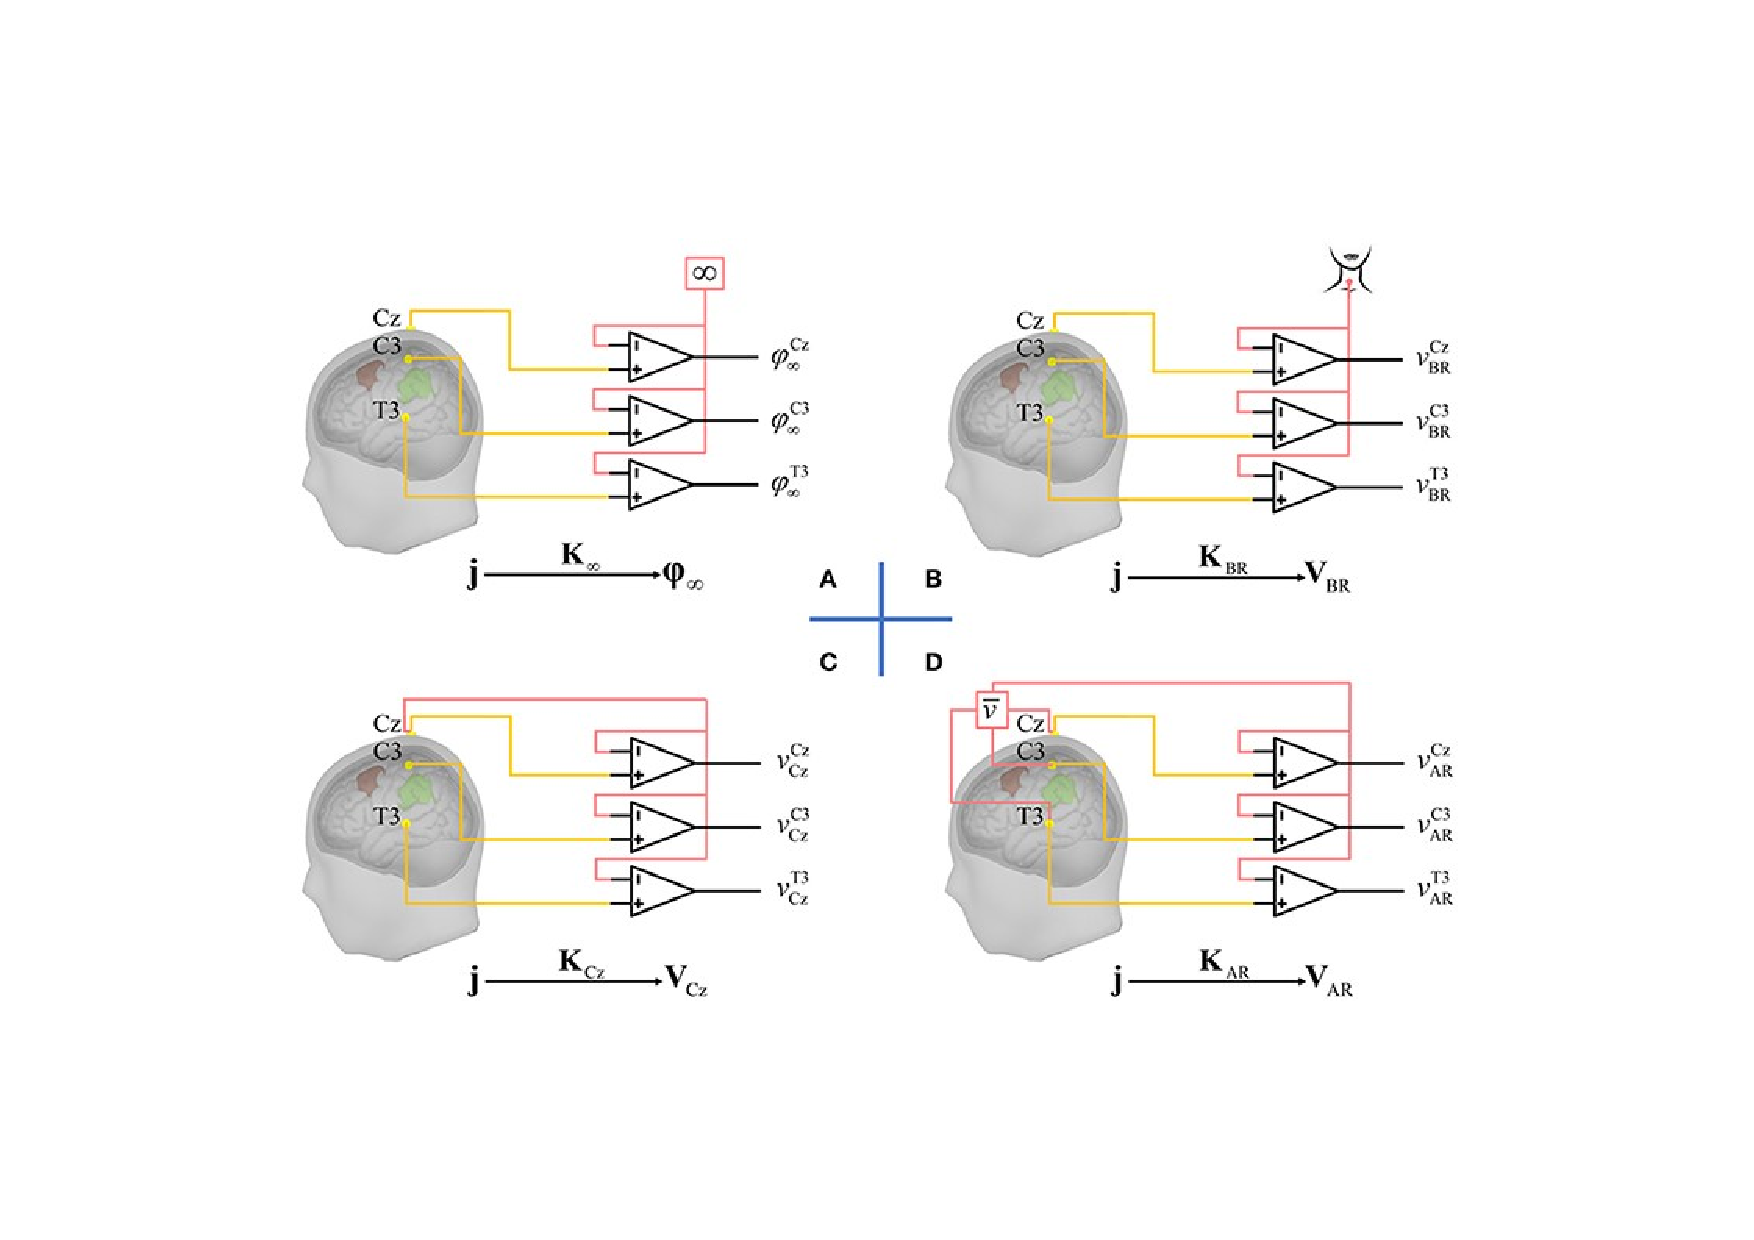
\includegraphics[width=0.8\textwidth,natwidth=610,natheight=642]{pic/3.1.pdf}
\end{figure}


\section{结果}

\section{本章小结}
我们研究发现脑电参考问题可以统一为逆问题的一种,其可以通过贝叶斯技术解决。据我们所知,这是对脑电参考问题的一种创新方案,这允许我们:采用正则化方法估计无穷远参考下的电势,证明了无穷远参考和平均参考是统一贝叶斯估计量的特例只是二者区别于脑电电势的空间协方差先验,同时引入去噪进入参考估计程序中,采用了模型选择准则来选择最优的参考估计量。模型选择的结果归纳为:正则化的参考(无穷远或者平均)优于传统的无穷远或平均参考,其中正则化的无穷远参考无论在仿真研究还是真实数据验证上都体现了最优的性能;容积传导模型的选择是基于被试个体的传递矩阵或者被试群体平均的传递矩阵。
在本章中,我们采用贝叶斯最大后验估计,发现无穷远参考和平均参考属于统一的统计学架构,其区别在于先验的不同,采用基于容积传导的头表电极协方差先验和无噪声理想情况下得到的是无穷远参考,采用独立同分布的头表电极协方差在无噪声情况下得到的是平均参考,有噪声的情况下均视为正则化的参考电极标准化技术。这种技术称为rREST,作为无穷远参考的脑电电势的改进的估计量,有希望在临床实践中得以推广使用。